Per poter assicurare una conduzione e uno sviluppo del progetto che soddisfino le scadenze, il gruppo ha deciso di ripartire il lasso di tempo che va dalla sua formazione fino alla revisione di accettazione nelle seguenti cinque attività:

\begin{itemize}
	\item analisi dei requisiti;
	\item consolidamento dei requisiti;
	\item progettazione della \glock{technology baseline};
	\item progettazione di dettaglio e codifica;
	\item validazione e collaudo.
\end{itemize}
Ogni attività verrà poi frammentata in altri sotto periodi, in ognuno dei quali verrà associata una \glock{milestone},
riferita alla data di fine periodo, per il completamento delle singole attività previste al suo interno.\\
In un intervallo di tempo vengono quindi inserite più attività, le quali, possono essere svolte sia sequenzialmente, sia con un certo grado di parallelismo in base alle dipendenze che sussistono tra di loro.

\subsection{Analisi dei requisiti}
L’attività di analisi dei requisiti ha inizio il giorno 31-10-2020, successivamente alla formazione dei gruppi, suddivisa in cinque periodi, con termine fissato per il giorno 11-01-2020, giorno di consegna dei documenti in ingresso alla revisione dei requisiti.

\subsubsection{Ruoli attivi}
Durante questa attività è necessaria la presenza dei seguenti ruoli:
\begin{itemize}
	\item Responsabile;
	\item amministratore;
	\item analista;
	\item verificatore.
\end{itemize}

\subsubsection{Periodi}
L'attività di analisi dei requisiti è stata suddivisa nei seguenti cinque periodi:

\paragraph{Primo periodo dal 31-10-2020 al 05-12-2020}
\begin{itemize}
	\item \textbf{Analisi dei capitolati}: studio individuale dei \glock{capitolati} e discussione interna al gruppo dei pregi e svantaggi individuati da ogni componente, in modo da indirizzare l’interesse del gruppo su certi \glock{capitolati} piuttosto che su altri;
	\item \textbf{ricerca}: individuazione e studio degli strumenti e delle tecnologie di supporto da utilizzare per la gestione del progetto;
	\item \textbf{studio di fattibilità}: impostato sulla base dell'analisi dei \glock{capitolati} fatta in precedenza;
	\item \textbf{pianificazione attività}: decisione dell'organizzazione interna al gruppo riguardo i ruoli da assegnare ed i compiti da svolgere.
\end{itemize}

\paragraph{Secondo periodo dal 05-12-2020 al 17-12-2020}
\begin{itemize}
	\item \textbf{Scelta del capitolato}: decisione definitiva riguardo il \glock{capitolato} scelto;
	\item \textbf{normazione}: scelta delle regole da adottare durante lo sviluppo del progetto riguardanti i processi primari e processi organizzativi;
	\item \textbf{studio di fattibilità}: fine dello \dext{Studio di fattibilità v1.0.0}, basato sul \glock{capitolato} scelto.
\end{itemize}

\paragraph{Terzo periodo dal 18-12-2020 al 29-12-2020}
\begin{itemize}
	\item \textbf{Analisi dei casi d'uso}: analisi del prodotto e dei casi d’uso;
	\item \textbf{norme di progetto}: stesura delle \dext{Norme di progetto v1.0.0};
	\item \textbf{piano di progetto}: stesura del \dext{Piano di progetto v1.0.0};
	\item \textbf{analisi dei rischi}: individuazione dei rischi che possono presentarsi nello svolgimento del progetto.
\end{itemize}

\paragraph{Quarto periodo dal 30-12-2020 al 07-01-2021}
\begin{itemize}
	\item \textbf{Analisi dei requisiti}: stesura dell’\dext{Analisi dei requisiti v1.0.0};
	\item \textbf{piano di qualifica}: stesura del \dext{Piano di qualifica v1.0.0};
	\item \textbf{glossario}: stesura del \dext{Glossario v1.0.0}.
\end{itemize}

\paragraph{Quinto periodo dal 08-01-2021 al 11-01-2021}
\begin{itemize}
	\item \textbf{Revisione}: ultimo controllo di tutti i documenti scritti;
	\item \textbf{presentazione RR}: presentazione della revisione dei requisiti.
\end{itemize}


\newpage

\begin{landscape}
	\begin{figure}[h!]
		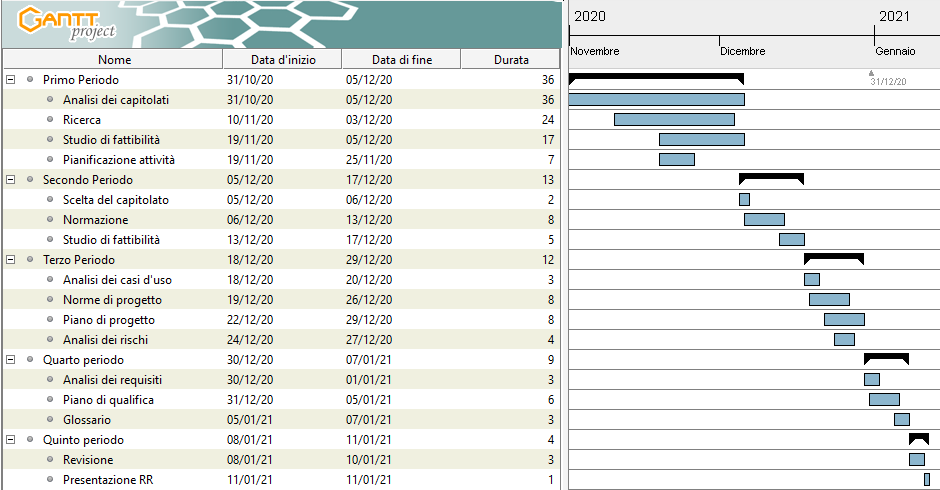
\includegraphics[width=24cm]{images/1_Analisi_dei_requisiti.png}
		\caption{Pianificazione - Analisi dei requisiti}
	\end{figure}
\end{landscape}

\newpage

\subsection{Consolidamento dei Requisiti}
L'attività di consolidamento dei requisiti ha inizio il giorno 12-01-2021, successivamente alla consegna del materiale in ingresso alla revisione dei requisiti, suddivisa in due periodi, con termine fissato
per il giorno 17-01-2021 che precede la revisione dei requisiti del 18-01-2021.

\subsubsection{Ruoli attivi}
Durante questa attività è necessaria la presenza dei seguenti ruoli:
\begin{itemize}
	\item Responsabile;
	\item amministratore;
	\item analista.
\end{itemize}

\subsubsection{Periodi}
L'attività di consolidamento dei requisiti è stata suddivisa nei seguenti due periodi:

\paragraph{Primo periodo dal 12-01-2021 al 15-01-2021}
\begin{itemize}

	\item \textbf{Preparazione presentazione}: redazione della presentazione da portare in sede di revisione e studio individuale.

\end{itemize}

\paragraph{Secondo periodo dal 16-01-2021 al 17-01-2021}
\begin{itemize}

	\item \textbf{Analisi dei requisiti}: revisione ed eventuale aggiornamento dei requisiti.

\end{itemize}

\newpage

\begin{landscape}
	\begin{figure}[h!]
		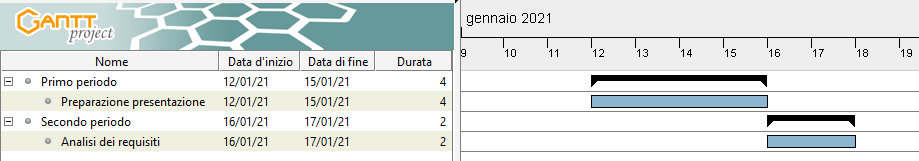
\includegraphics[width=24cm]{images/2_Consolidamento_dei_requisiti.png}
		\caption{Pianificazione - Consolidamento dei requisiti}
	\end{figure}
\end{landscape}

\newpage
\subsection{Codifica della \glock{Technology Baseline}}
L'attività di codifica della \glock{technology baseline} ha inizio il giorno 01-02-2021, successivamente alla revisione dei requisiti, suddivisa in quattro periodi, con termine fissato per il giorno 14-03-2021 che precede la revisione di progettazione del 15-03-2021.

\subsubsection{Ruoli attivi}
Durante questa attività è necessaria la presenza dei seguenti ruoli:
\begin{itemize}
	\item Responsabile;
	\item amministratore;
	\item analista;
	\item progettista;
	\item programmatore;
	\item verificatore.
\end{itemize}

\subsubsection{Periodi}
L'attività di progettazione della \glock{technology baseline} è stata suddivisa nei seguenti periodi:

\paragraph{Primo periodo dal 01-02-2021 al 10-02-2021}
\begin{itemize}
	\item \textbf{Normazione}: revisione ed eventuale aggiornamento delle norme;
	\item \textbf{aggiornamento della pianificazione};
	\item \textbf{aggiornamento della qualità};
	\item \textbf{analisi dei requisiti}: revisione ed eventuale aggiornamento dei casi d’uso e dei requisiti, in base alle indicazioni ricevute;
	\item \textbf{ricerca}: studio autonomo degli strumenti e le tecnologie da utilizzare per lo sviluppo del
	progetto;
	\item \textbf{verifica}: controllo della qualità di tutti i prodotti sviluppati durante il periodo attuale.
\end{itemize}

\paragraph{Secondo periodo dal 19-02-2021 al 06-03-2021}
\begin{itemize}
	\item \textbf{Normazione}: aggiornamento delle norme;
	\item \textbf{progettazione}: progettazione del \glock{proof of concept} che deve essere implementato;
	\item \textbf{codifica}: implementazione del \glock{proof of concept} progettato;
	\item \textbf{verifica}: controllo della qualità di tutti i prodotti sviluppati durante il periodo attuale.
\end{itemize}

\paragraph{Terzo periodo dal 09-03-2021 al 14-03-2021}
\begin{itemize}
		\item \textbf{Stesura della lettera di presentazione}: scrittura della lettera di presentazione con la quale ci
	si candida alla revisione di progettazione;
		\item \textbf{aggiornamento documentazione};
	\item \textbf{verifica}:controllo della qualità di tutti i prodotti sviluppati durante il periodo attuale.
\end{itemize}

\paragraph{Quarto periodo dal 15-03-2021 al 20-03-2021}
\begin{itemize}
	\item \textbf{Preparazione presentazione}: redazione della presentazione da portare in sede di revisione e
	studio individuale.
\end{itemize}

\newpage
\begin{landscape}
	\begin{figure}[h!]
		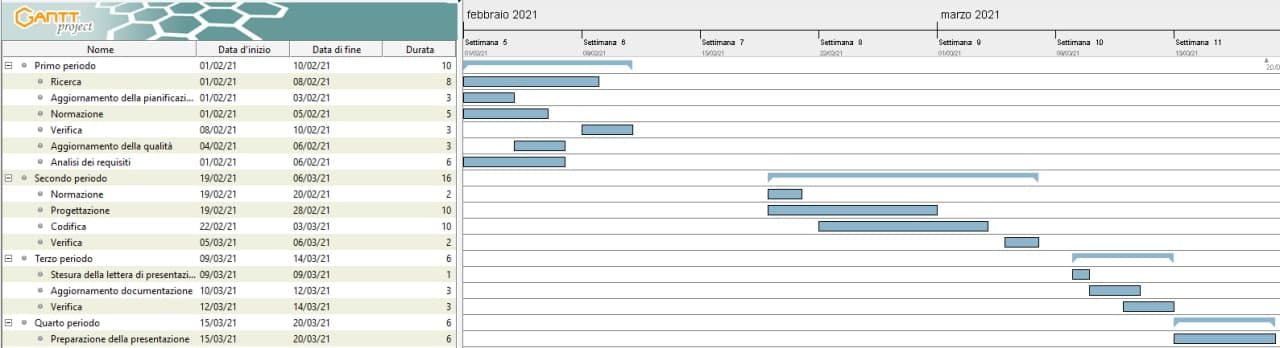
\includegraphics[width=24cm]{images/tb.jpg}
		\caption{Pianificazione - Codifica \glock{Technology baseline}}
	\end{figure}
\end{landscape}

 \newpage

 \subsection{Incrementi}
 Di seguito la pianificazione si baserà sugli incrementi ognuno dei quali ha una data di fine e di inizio. Alcuni incrementi potranno essere eseguiti in parallelo ed assegnati ad un sottogruppo appositamente creato. \\
  L'obiettivo di ogni incremento è creare nuove funzionalità e, di fatti; la loro realizzazione è affine ai requisti funzionali ed i relativi test descritti rispettivamente in \dext{Analisi dei requisiti v2.0.0} e \dext{Piano di qualifica v2.0.0}.\\
 Tale pianificazione apporta una nuova stesura dei preventivi.

 \subsubsection{Incremento I}
  \begin{itemize}
  	\item \textbf{Periodo}: dal 22-03-2021 al 29-03-2021;
  	\item \textbf{Assegnatari}: Gruppo I;
  	\item \textbf{Funzionalità}:
  		\begin{itemize}
  		\item creazione lista utenti;
  		\item creazione lista unità.
  	    \end{itemize}
  \end{itemize}

 \subsubsection{Incremento II}
 \begin{itemize}
 	\item \textbf{Periodo}: dal 22-03-2021 al 29-03-2021;
 	\item \textbf{Assegnatari}: Gruppo II;
 	\item \textbf{Funzionalità}:
 	\begin{itemize}
 		\item creazione interfaccia Login/Logout.
 	\end{itemize}
 \end{itemize}

\subsubsection{Incremento III}
\begin{itemize}
	\item \textbf{Periodo}: dal 30-03-2021 al 06-04-2021;
	\item \textbf{Assegnatari}: tutto il gruppo;
	\item \textbf{Funzionalità}:
	\begin{itemize}
		\item definizione realizzazione dei permessi:
		\begin{itemize}
			\item tra diversi tipi di utenti;
			\item rapporto utenti ed unità;
			\item tra utenti e sistema.
		\end{itemize}
	\end{itemize}
\end{itemize}


 \subsubsection{Incremento IV}
\begin{itemize}
	\item \textbf{Periodo}: dal 07-04-2021 al 17-04-2021;
	\item \textbf{Assegnatari}: Gruppo I;
	\item \textbf{Funzionalità}:
	\begin{itemize}
	\item coda ordini: ogni unità ha una coda che rappresenta i punti di interesse in cui stazionare per eseguire ogni ordine.
	\end{itemize}
\end{itemize}

 \subsubsection{Incremento V}
\begin{itemize}
	\item \textbf{Periodo}: dal 07-04-2021 al 17-04-2021;
	\item \textbf{Assegnatari}: Gruppo II;
	\item \textbf{Funzionalità}:
	\begin{itemize}
		\item ostacoli accidentali: l'unità è in grado di ricevere un nuovo percorso nel momento in cui è in grado di rilevare un ostacolo non previsto.
	\end{itemize}
\end{itemize}
\subsubsection{Incremento VI}
\begin{itemize}
	\item \textbf{Periodo}: dal 20-04-2021 al 27-04-2021;
	\item \textbf{Assegnatari}: Gruppo I;
	\item \textbf{Funzionalità}:
	\begin{itemize}
		\item stato unità: l'unità possiede i seguenti stati:
		\begin{itemize}
			\item Going to X;
			\item Stop;
			\item Base;
			\item Error Y.
		\end{itemize}
	\end{itemize}
\end{itemize}

\subsubsection{Incremento VII}
\begin{itemize}
	\item \textbf{Periodo}: dal 20-04-2021 al 27-04-2021;
	\item \textbf{Assegnatari}: Gruppo II;
	\item \textbf{Funzionalità}:
	\begin{itemize}
		\item aggiornamento mappa tramite inserimento file apposito.
	\end{itemize}
\end{itemize}

\subsubsection{Incremento VIII}
\begin{itemize}
	\item \textbf{Periodo}: dal 01-05-2021 al 13-05-2021;
	\item \textbf{Assegnatari}: Gruppo I;
	\item \textbf{Funzionalità}:
	\begin{itemize}
		\item stesura Manuale utente.
	\end{itemize}
\end{itemize}

\subsubsection{Incremento IX}
\begin{itemize}
	\item \textbf{Periodo}: dal 01-05-2021 al 13-05-2021;
	\item \textbf{Assegnatari}: Gruppo II;
	\item \textbf{Funzionalità}:
	\begin{itemize}
		\item stesura Guida utente.
	\end{itemize}
\end{itemize}

\newpage

\begin{landscape}
	\begin{figure}[h!]
		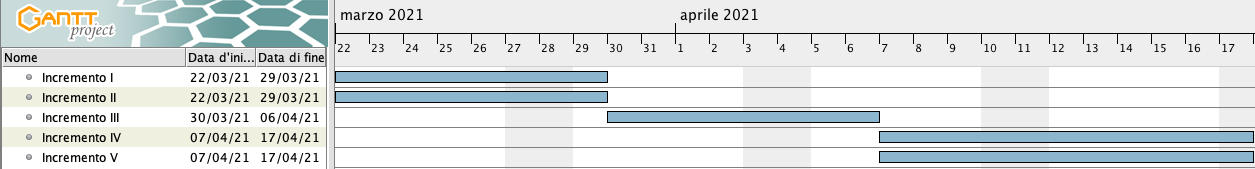
\includegraphics[width=24cm]{images/4_Incrementi_1.png}
		\caption{Pianificazione per incrementi - Prima parte}
	\end{figure}

    \begin{figure}[h!]
        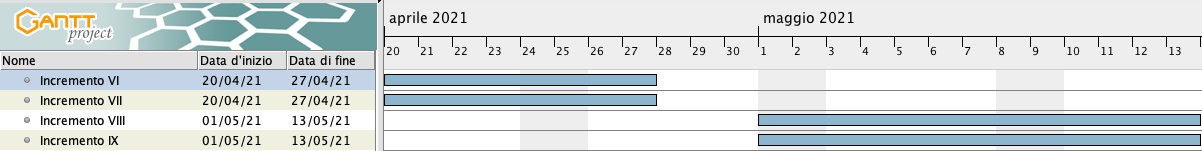
\includegraphics[width=24cm]{images/4_Incrementi_2.png}
        \caption{Pianificazione per incrementi - Seconda parte}
    \end{figure}
\end{landscape}

\newpage

\subsection{Validazione e collaudo}
L'attività di validazione e collaudo ha inizio il giorno 17-05-2021, successivamente alla revisione di qualifica, formato da un unico periodo, con termine fissato per il giorno 23-05-2021.

\subsubsection{Ruoli attivi}
Durante questa attività è necessaria la presenza dei seguenti ruoli:
\begin{itemize}
	\item Responsabile;
	\item amministratore;
	\item progettista;
	\item programmatore;
	\item verificatore.
\end{itemize}
\subsubsection{Periodi}
L'attività di validazione e collaudo è stata suddivisa nei seguenti periodi:
\paragraph{Primo periodo dal 17-05-2021 al 23-05-2021}
\begin{itemize}
	\item \textbf{Normazione}: revisione ed eventuale aggiornamento delle norme;
	\item \textbf{aggiornamento} della pianificazione;
	\item \textbf{aggiornamento della qualità};
	\item \textbf{completamento progettazione};
	\item \textbf{verifica}: controllo della qualità di tutti i prodotti sviluppati durante il periodo attuale;
	\item \textbf{preparazione presentazione}: redazione della presentazione da portare in sede di revisione e
	studio individuale.
\end{itemize}